\documentclass{beamer}
\usepackage{fancyvrb}
\usepackage{color}
\usepackage{hyperref}
\hypersetup{
  colorlinks = false,
  urlcolor = blue,
  pdfauthor = {Alexander Mazurov},
  pdfkeywords = {scientific computing, system and distributing programming},
  pdftitle = {Optimization of software trigger and chib studies in LHCb}
  pdfsubject = {Optimization of software trigger and chib studies in LHCb},
  pdfpagemode = UseNone
}
% ============================================================================
\title[Optimization and  $\chi_b$ studies]{Optimization of software trigger and $\chi_b$ studies in LHCb}
\subtitle{2nd year report}
\institute[University of Ferrara]{
  Department of Physics\\
  University of Ferrara, Italy\\
  \&\\
  LHCb experiment, CERN, Switzerland\\
  \texttt{alexander.mazurov@cern.ch}
}
% ============================================================================
\author[Sasha Mazurov]{Alexander (Sasha) Mazurov}
\date{30 November 2012}
\usetheme{Copenhagen}
\useoutertheme{infolines}
% ============================================================================
\begin{document}

\maketitle
\section{Introduction}
% ============================================================================
\begin{frame}
% ----------------------------------------------------------------------------
\frametitle{About Me}
\begin{columns}[c]
\column{.5\textwidth}
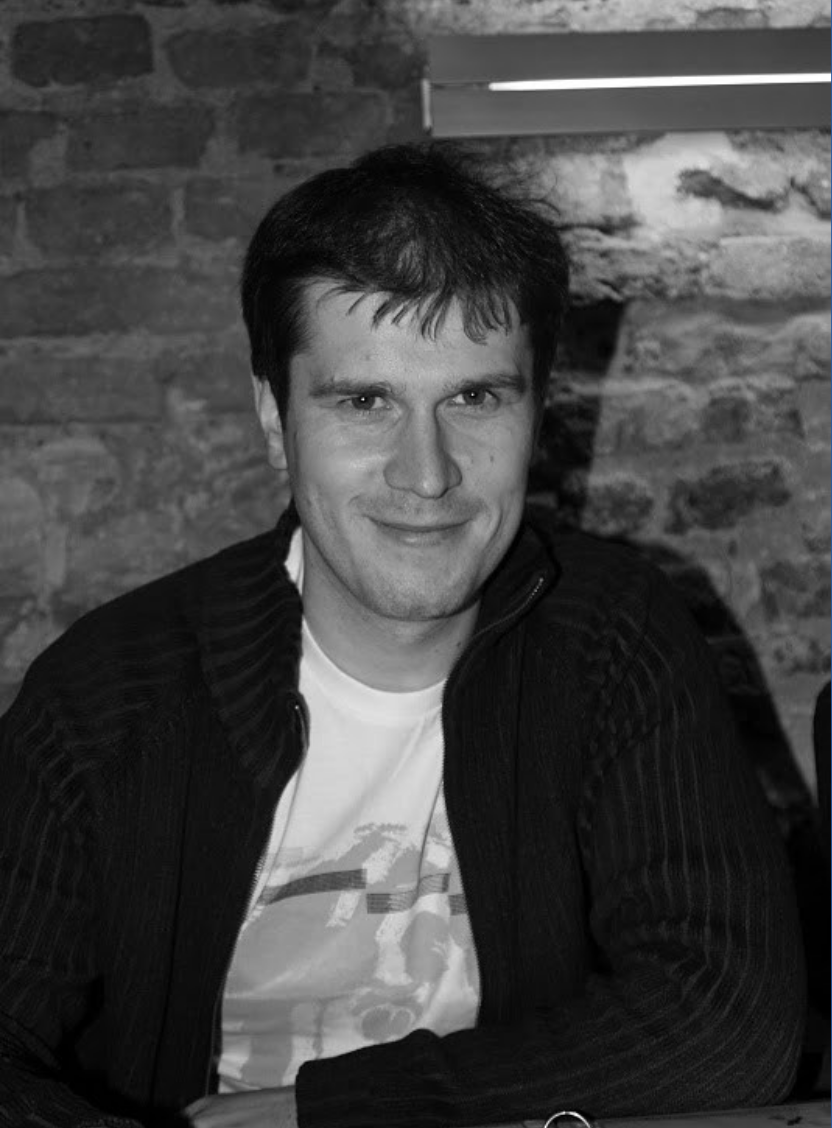
\includegraphics[width=.8\textwidth]{images/me.png}
\column{.5\textwidth}
\begin{itemize}
    \item From Protvino, Russia.
    \item {\bf 1997-2002:} Lomonosov's Moscow State University, MS Calculate
    Mathematic and System programming.
    \item {\bf 2007-present:} CERN, LHCb experiment.
\end{itemize}
\end{columns}
% ----------------------------------------------------------------------------
\end{frame}
% ============================================================================
\begin{frame}[t]
% ----------------------------------------------------------------------------
\frametitle{LHCb experiment (1)}
\begin{itemize}
  \item One of the four largest experiments in Large Hadron Collider (LHC)
  \item 843 members, from 60 institutes in 16 Countries
\end{itemize}
\begin{columns}[t]
\column{.5\textwidth}
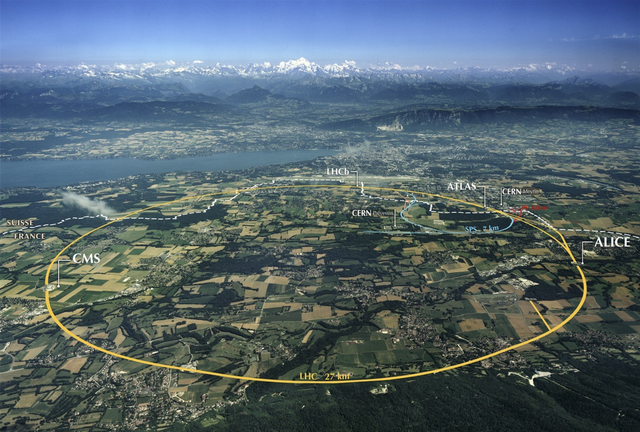
\includegraphics[width=\textwidth]{images/lhcb.png}
\column{.5\textwidth}
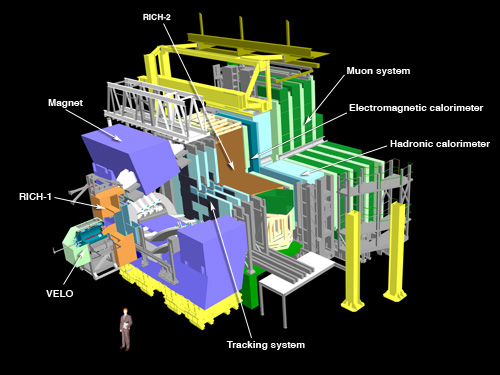
\includegraphics[width=\textwidth]{images/det.png}\\~\\
Forward spectrometer.
\end{columns}

% ----------------------------------------------------------------------------
\end{frame}
% ============================================================================
\begin{frame}
% ----------------------------------------------------------------------------
\frametitle{LHCb experiment (2)}
Core physics program is a searching for NEW physics with Charm and Beauty particles.
\begin{columns}[c]
\column{.5\textwidth}
\begin{alertblock}{Hot result (November 2012)}
First evidence for the $B^{0}_{s} \rightarrow \mu^+ \mu^-$ decay.
Branching:  $3.2^{+1.5}_{-1.2} \times 10^{-9}$.
\end{alertblock}
Consistent with Standard Model
\column{.5\textwidth}
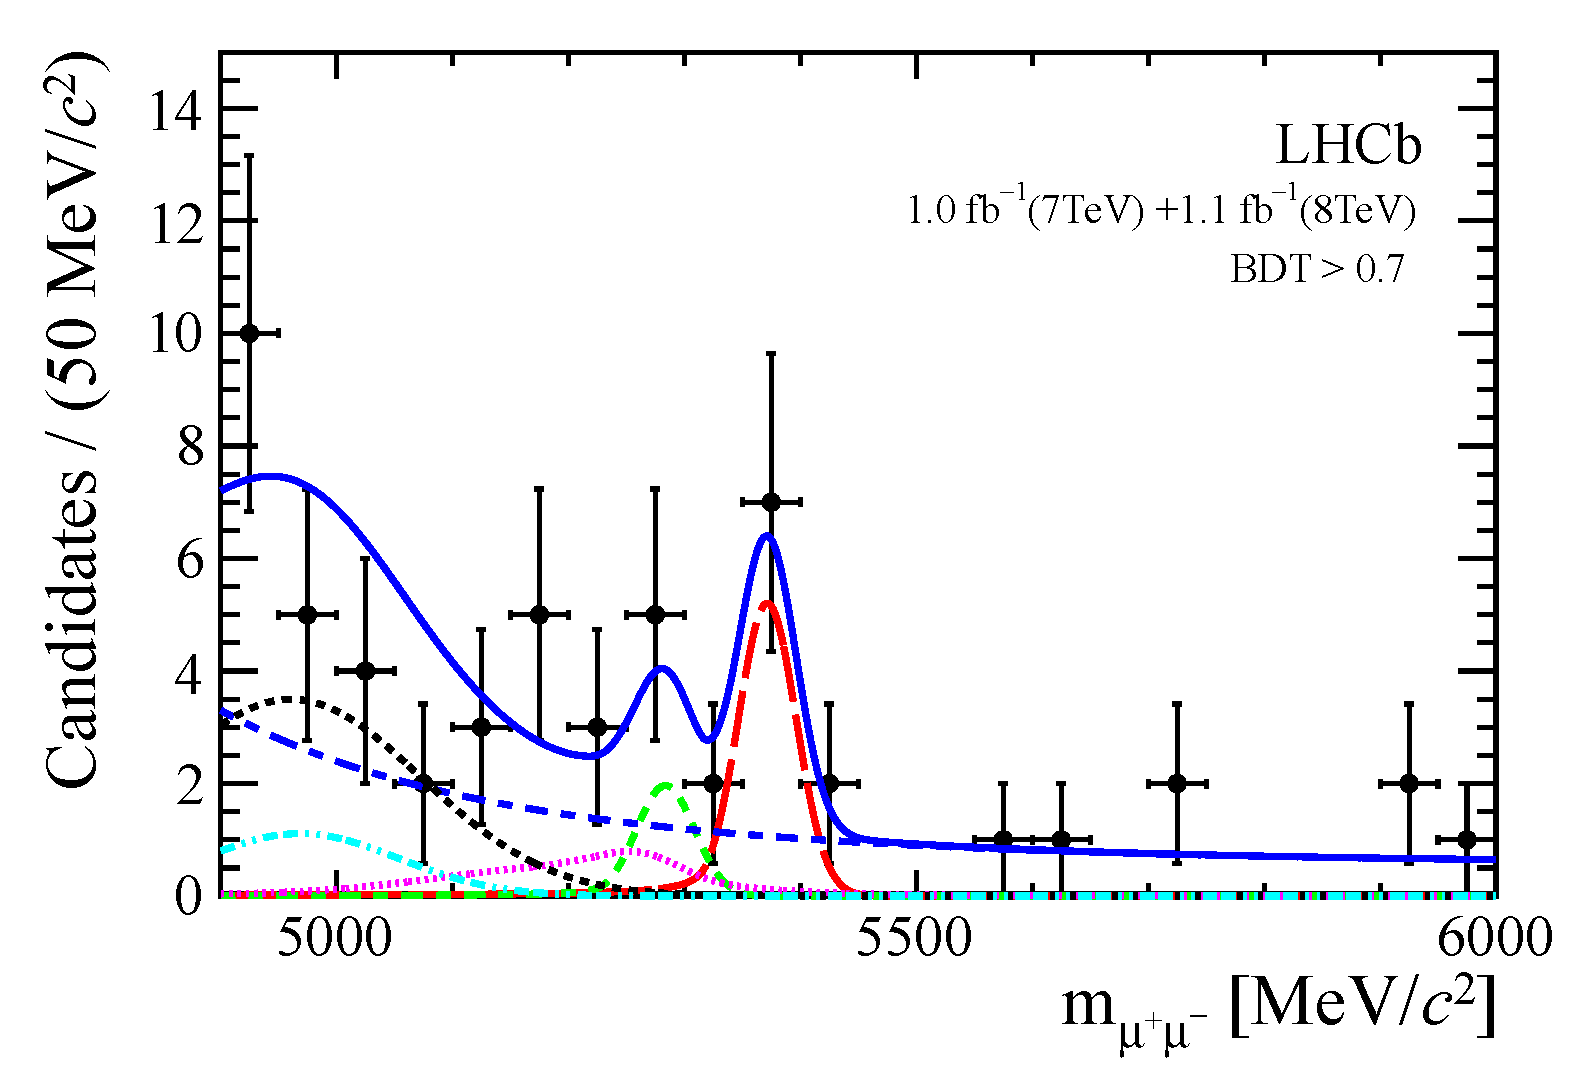
\includegraphics[width=\textwidth]{images/bs.png}
\end{columns}
\begin{itemize}
 \item Many experiments have been looking for this decay in the last 10 years.
 \item LHCb is the first to observe it!
\end{itemize}
% ----------------------------------------------------------------------------
\end{frame}
% ============================================================================
\begin{frame}
% ----------------------------------------------------------------------------
\frametitle{My research}
\begin{enumerate}
    \item Trigger software profiling. \textcolor{green}{DONE}
    \item Study of $\chi_{b}$ production. \textcolor{blue}{IN PROGRESS}
\end{enumerate}
% ----------------------------------------------------------------------------
\end{frame}
% ============================================================================
\section{Trigger software profiling}
\begin{frame}
\begin{exampleblock}{}
  \begin{center}
    {\huge Trigger software profiling}
  \end{center}
\end{exampleblock}

\end{frame}

\begin{frame}
\frametitle{Trigger software profiling}
\begin{columns}[c]
\column{.4\textwidth}
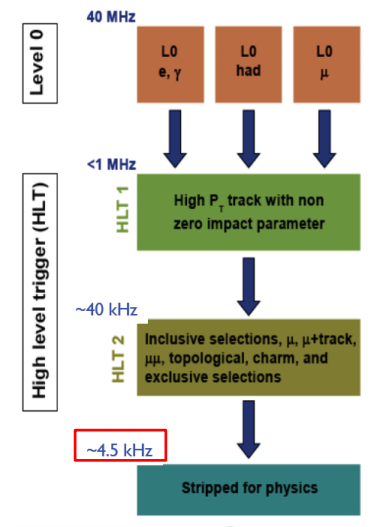
\includegraphics[width=.9\textwidth]{images/hlt_struct1.png}\\~\\
\textcolor{red}{The trigger needs fast algorithms!}
\column{.6\textwidth}
Most experiments require a trigger in order to record interesting events at suitable rate.
\begin{itemize}
  \item L0 Hardware Trigger $40 MHz \rightarrow 1 MHz$. Search for high pt, $\mu$, e, $\gamma$, hadron candidates.
  \item High Level Software Trigger Farm
  \begin{itemize}
    \item HLT1: Add Impact parameter cuts
    \item HLT2: Global event reconstruction.
  \end{itemize}
\end{itemize}
\begin{itemize}
  \item 100 man/years work that has only 20-30 ms to process an average event.
  \item 29K CPUs or 1700 servers.
  \item $2 \times 10^{15}$ bytes stored in 2012.
\end{itemize}
% 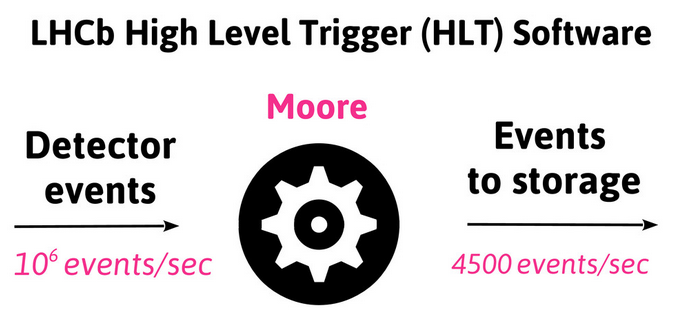
\includegraphics[width=.8\textwidth]{images/moore.png}
\end{columns}
\end{frame}
\subsection{Profiler Auditor}
\begin{frame}
\frametitle{CPU Profiler Auditor}
CPU profiler tool is vital for trigger optimization.\\~\\
\begin{columns}[c]
\column{.5\textwidth}
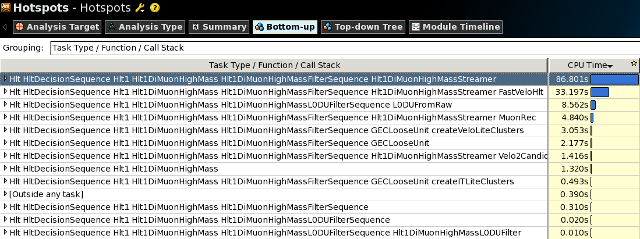
\includegraphics[width=\textwidth]{images/cpu01.png}\\~\\
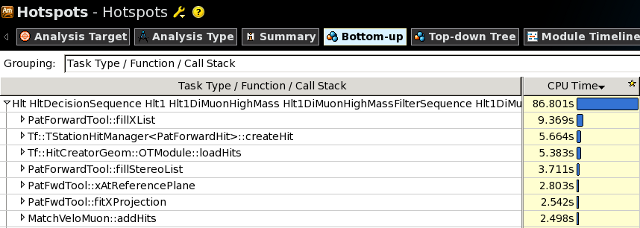
\includegraphics[width=\textwidth]{images/cpu02.png}
\column{.5\textwidth}
\begin{itemize}
    \item C++ library.
    \item Deployed into the core software framework in LHCb --- Gaudi.
    \item Based on Intel\textsuperscript{\textregistered} VTune\texttrademark
    Amplifier XE User API
    \item Full and clear reports.
\end{itemize}
\end{columns}
\end{frame}

\begin{frame}
\frametitle{Example of trigger hotspot}
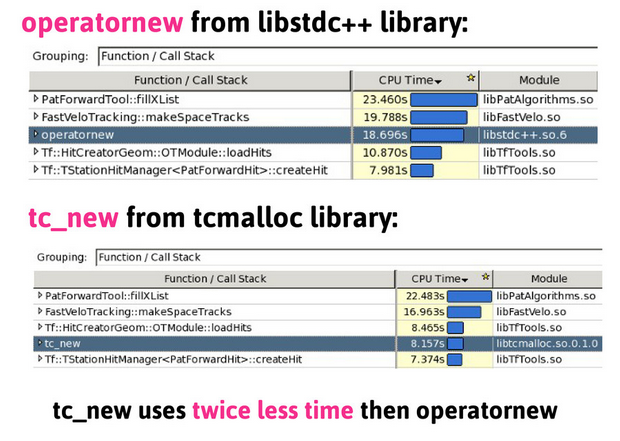
\includegraphics[width=.7\textwidth]{images/hlt.png}\\~\\
\begin{itemize}
  \item Hotspot was found.
  \item Allows to decrease CPU consumption by 5\%.
\end{itemize}
\end{frame}
\begin{frame}
\frametitle{CHEP2012: Talk and Paper}
This work was presented on "Computing in High Energy and Nuclear Physics" conference.
The largest of the conferenes in this area. The conference is held every 18 months.
\begin{columns}[l]
\column{.4\textwidth}
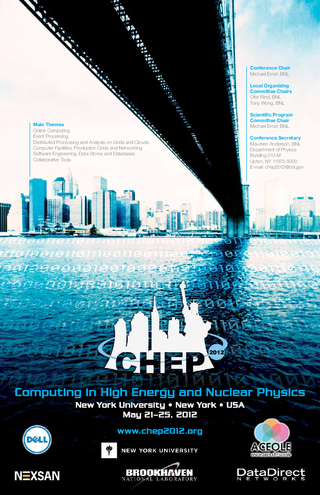
\includegraphics[height=.6\textheight]{images/chep.png}
\column{.6\textwidth}
\begin{itemize}
    \item Paper "Advanced Modular Software Performance Monitoring", Journal of Physics: Conference Series. Was accepted for publishing.
\end{itemize}
\end{columns}
\end{frame}
\section{Study of $\chi_{b}$ production}
\begin{frame}
\begin{exampleblock}{}
    \begin{center}
        {\huge Study of $\chi_{b}$ production}
    \end{center}
\end{exampleblock}
\end{frame}
% =============================================================================
\begin{frame}
Optimizing the LHCb trigger is crucial in many measurement. In particular,
decays with muons can be triggered on with \textbf{unprecedented high efficiency} ($\sim$80\%).
\begin{columns}[c]
\column{.5\textwidth}
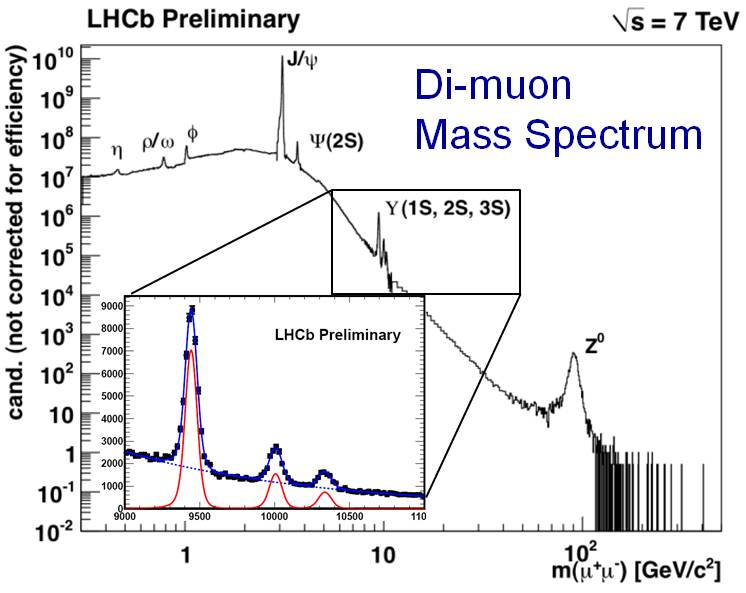
\includegraphics[width=\textwidth]{images/mumu.png}
\column{.5\textwidth}
The dimuon trigger:

\begin{itemize}
  \item is not prescaled.
  \item is used in more than 50\% of LHCb's papers.
\end{itemize}
\end{columns}
\end{frame}
% =============================================================================
\begin{frame}
\frametitle{Motivation and Plan}
$b\bar{b}$ system, which can be produced in different spin configurations, is ideal laboratory for QCD tests. It's like a hydrogen atom in QCD.
\begin{columns}[c]
\column{.3\textwidth}
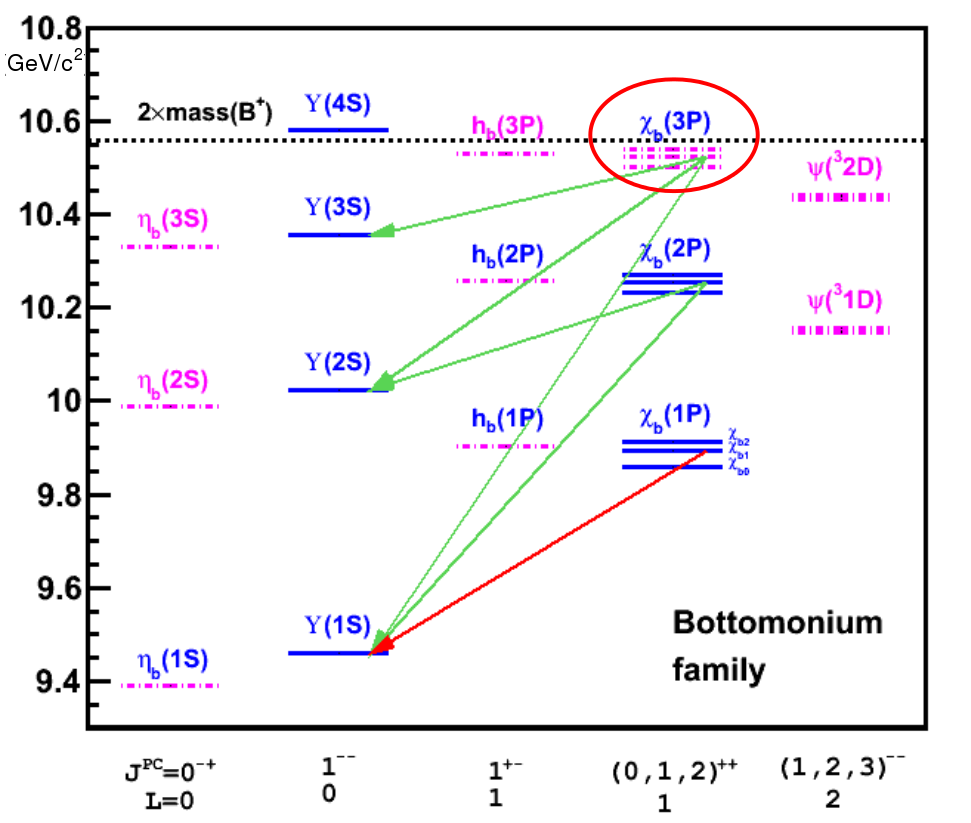
\includegraphics[width=\textwidth]{images/bfamily.png}
\begin{itemize}
  \item \textcolor{blue}{Measured mass}
  \item \textcolor{red}{Mass from theory}
\end{itemize}
\column{.7\textwidth}
States with parallel quark spins (S=1):
\begin{itemize}
  \item S-wave $\Upsilon$ state.
  \item P-wave $\chi_{b}$ states, composed by 3 spin states $\chi_{b(1,2,3)}$. Can be readily produced in the radiactive decays of $\Upsilon$.
  \item $\chi_{b}(3P)$ state recently observed by ATLAS, D0 and LHCb.
\end{itemize}
Study of $\chi_{b}$ production:
\begin{enumerate}
  \item Measurement for $\Upsilon(NS)$ (N=1, 2, 3) cross sections in $\chi_b$ decays as a function of $p_T(N\Upsilon)$
  \item Measurement of $\chi_{b(0,1,2)}(3P)$ mass.
\end{enumerate}
\end{columns}
\end{frame}
% =============================================================================
\subsection{Cross sections}
\begin{frame}
\frametitle{Cross sections formula}
In each $p_T(\Upsilon)$ bin calculate:
\begin{center}
$\frac{\sigma(\chi_{b} \rightarrow \Upsilon \gamma)}{\sigma(\Upsilon)} = \frac{N_{\chi_b \rightarrow \Upsilon \gamma}}{N_{\Upsilon}} \times \frac{\epsilon_{\Upsilon}}{\epsilon_{\chi_b \rightarrow \Upsilon \gamma}} = \frac{N_{\chi_b \rightarrow \Upsilon \gamma}}{N_{\Upsilon}} \times \frac{1}{\epsilon_{\gamma}^{reco}}$
\end{center}
\begin{itemize}
  \item Calculate for each $\Upsilon(nS), n=1,2,3$ and $\chi_b(mP), m=1,2,3$
  \item Get N from fits: $N_{\Upsilon}$ from  $m(\mu^+ \mu^-)$ and $N_{\chi_b \rightarrow \Upsilon \gamma}$ from [$m(\mu^+ \mu^- \gamma) - m(\mu^+ \mu^-)$] (for better resolution)
  \item Compute efficiency $\epsilon$  from Monte-Carlo simulation
  \item Luminosity = $1015 \pm 35 pb^{-1}$, data collected in year 2011.
\end{itemize}
\end{frame}

\begin{frame}[t]
\frametitle{Reconstruction}
Models were built on top of RooFit toolkit and unbinned maximum likelihood fits were performed.
\begin{columns}[t]
\column{.5\textwidth}
For $N_{\Upsilon}$:
invariant mass
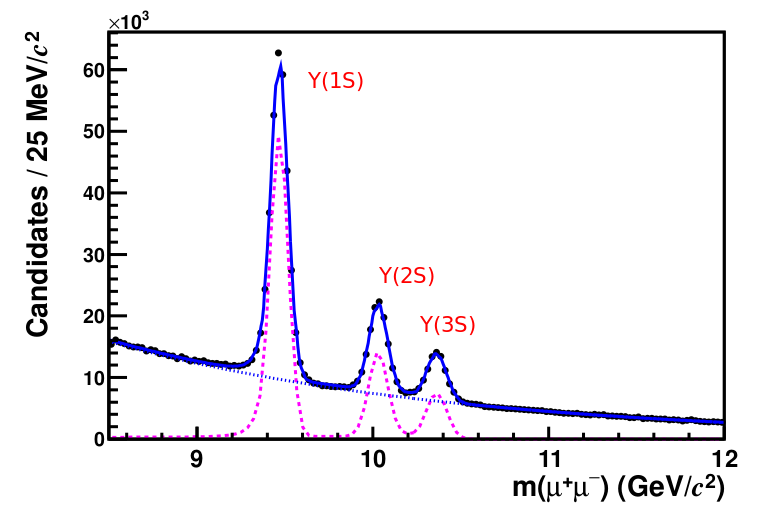
\includegraphics[height=.35\textheight]{images/ups.png}\\~\\
\begin{itemize}
  \item Signal: sum of 3 Crystal Ball functions
  \item Background: exponential function.
\end{itemize}
\column{.5\textwidth}
For $N_{\chi_{b} \rightarrow \Upsilon(1S) \gamma}$: mass difference
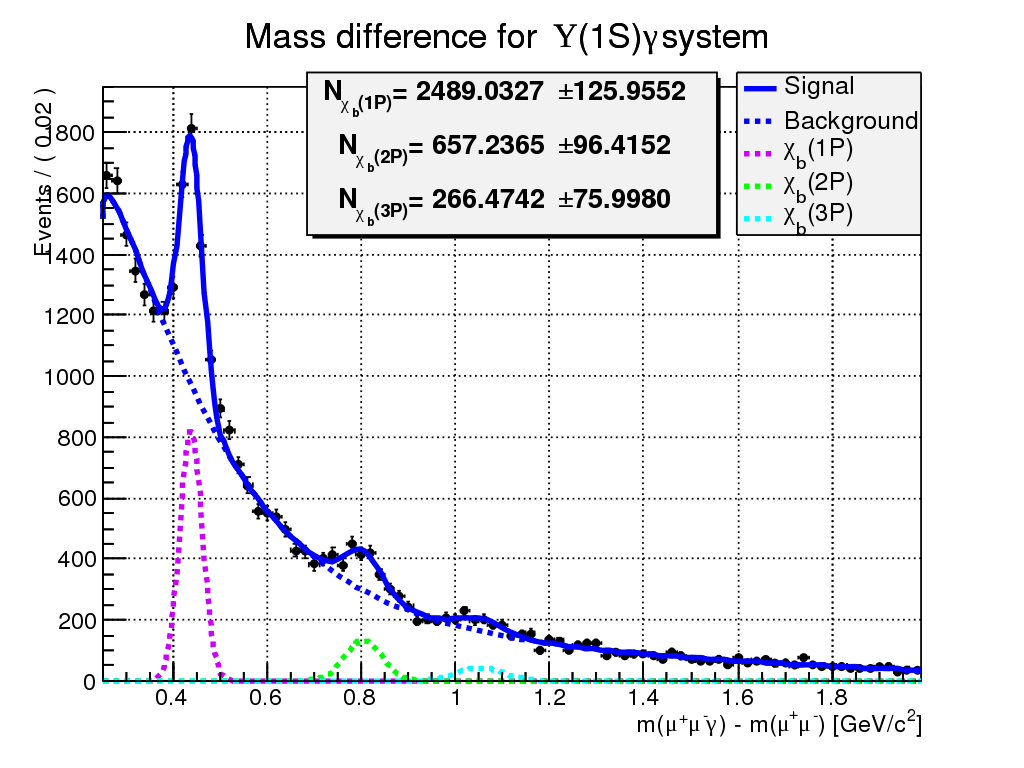
\includegraphics[height=.3\textheight]{images/fit.png}
\begin{itemize}
  \item Signal: 3 Gauss functions
  \item Background: $\sqrt{x} \times \left[e^{- \tau x} \times (c_1+a_1x+a_2x^2)\right] + \left[e^{-\tau x} \times (c_2+a_3x+a_4x^2)\right]$
\end{itemize}
(not enough resolution to separate $\chi_{b(0,1,2)}$)
\end{columns}
\end{frame}

\begin{frame}
\frametitle{Number of $\chi_b(NP) \rightarrow \Upsilon(1S)$ decays}
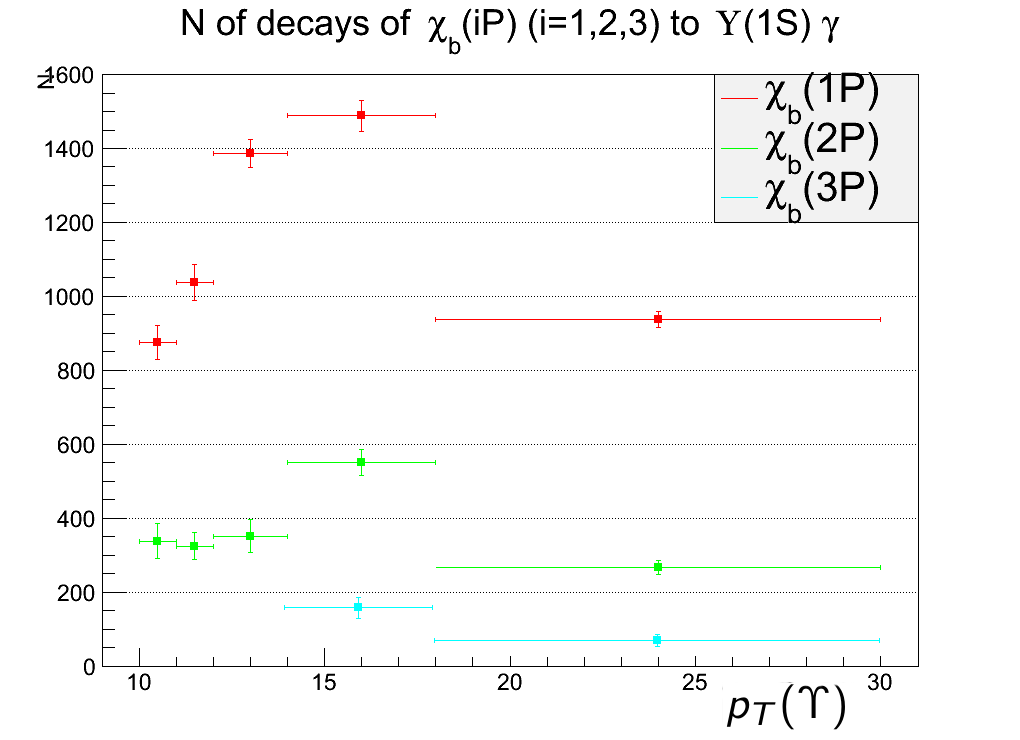
\includegraphics[width=.9\textwidth]{images/spectr.png}
\end{frame}
\subsection{Measurement of $\chi_{b}(3P)$ mass}
\begin{frame}
\begin{exampleblock}{}
    \begin{center}
        {\huge Measurement of $\chi_{b}(3P)$ mass}
    \end{center}
\end{exampleblock}
\end{frame}
\begin{frame}
\frametitle{Selection optimization}
Background subtraction
\begin{columns}[c]
\column{.5\textwidth}
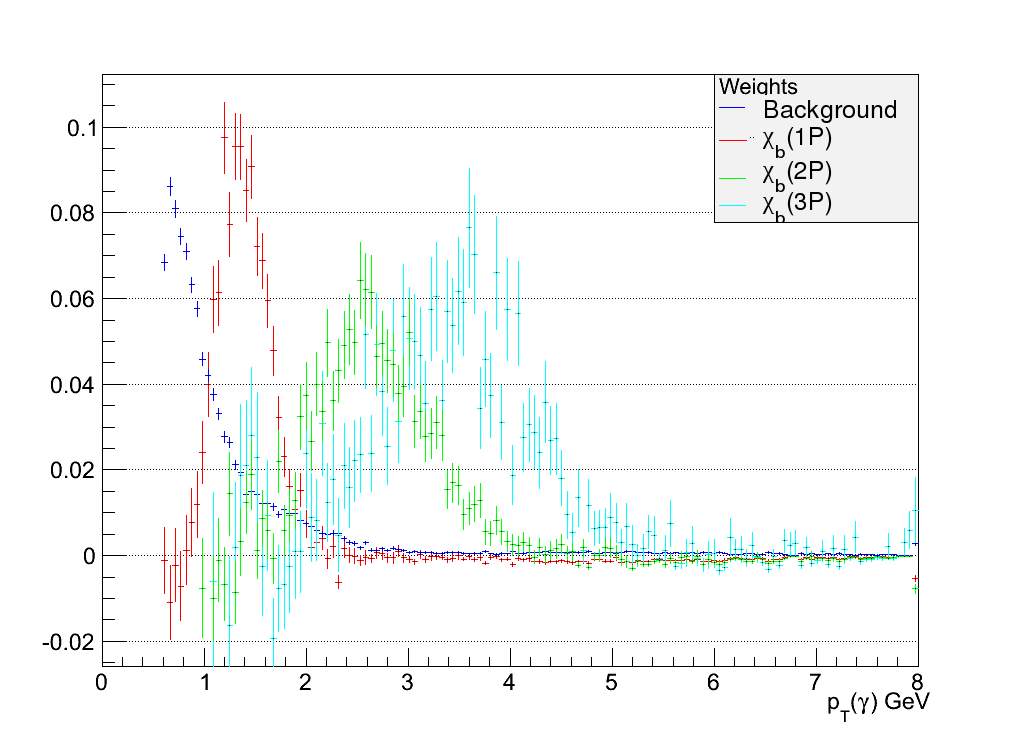
\includegraphics[width=\textwidth]{images/splot.png}
\column{.5\textwidth}
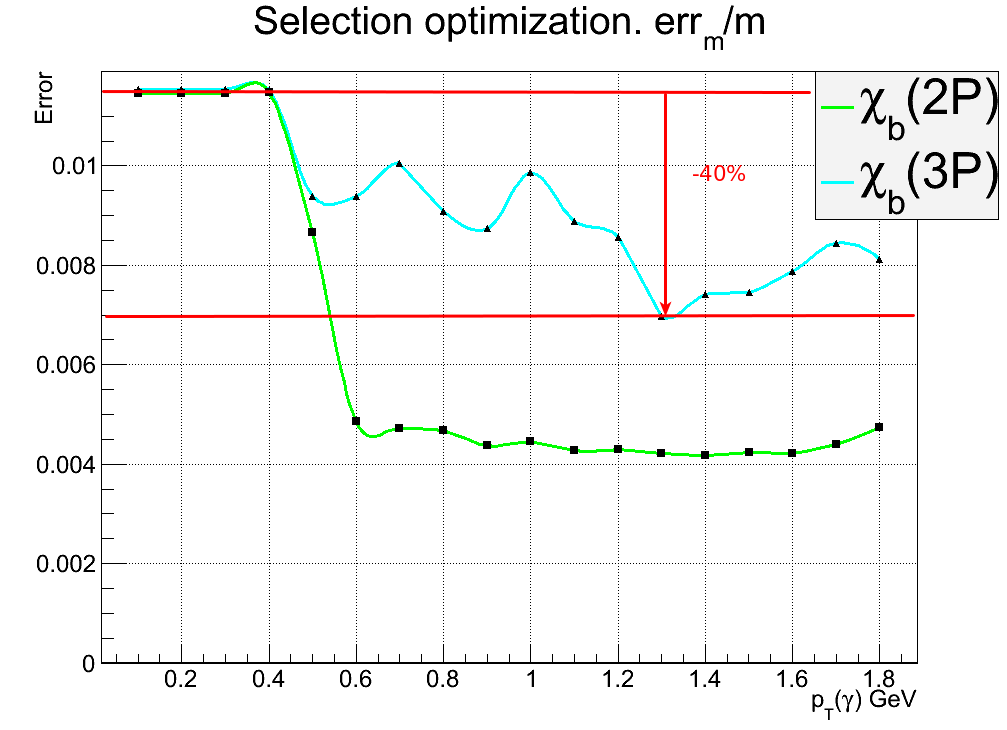
\includegraphics[width=\textwidth]{images/plot_rerr_m3p.png}
\end{columns}
\begin{itemize}
  \item We can reduce the background by tightening cut on $p_T(\gamma)$
  \item Can make a precise measurement of $m_{\chi_b(3P)}$
\end{itemize}
\end{frame}

\begin{frame}[t]
\frametitle{Very preliminary results}
\begin{columns}[T]
\column{.5\textwidth}
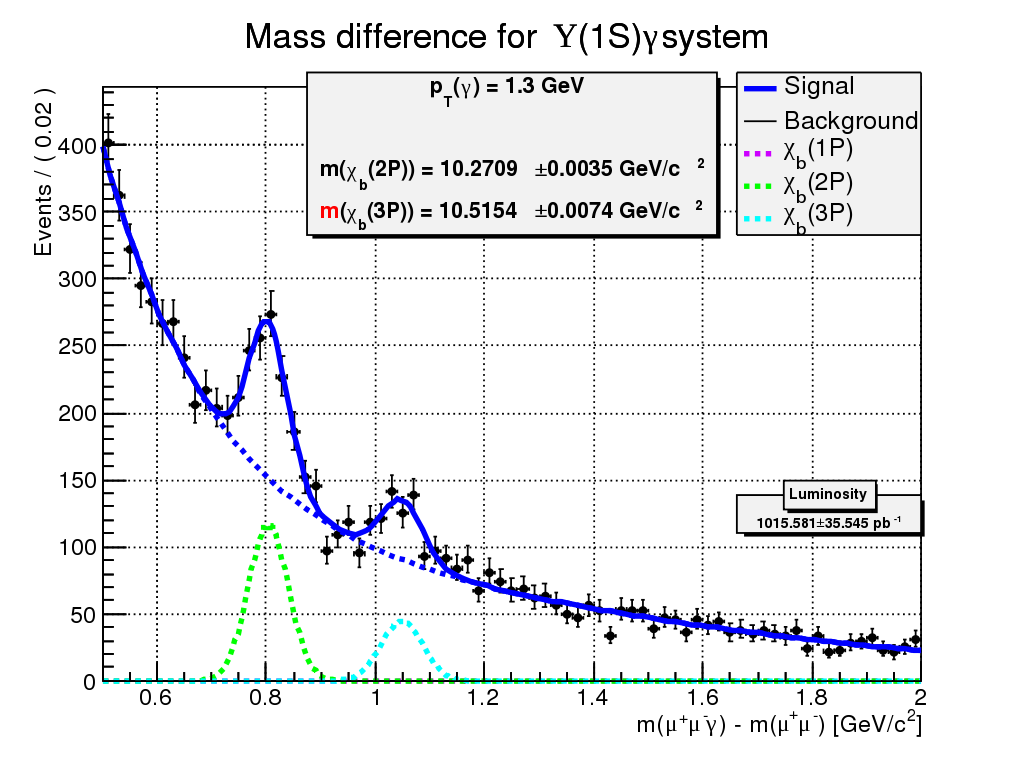
\includegraphics[height=.4\textheight]{images/m3p.png}\\~\\
\column{.5\textwidth}
Next steps:

\begin{itemize}
  \item Determine systematic errors
  \item Photon energy calibration
\end{itemize}
\end{columns}
\begin{tabular}{|l|c|c|}\hline
              &  $m_{\chi_b(2P)} [GeV/c^2]$ & $m_{\chi_b(3P)} [GeV/c^2]$\\ \hline
ATLAS         &                             & $10.530 \pm 0.0050$\\
D0            &                             & $10.551 \pm 0.0140$\\
LHCb (prev)   &  $10.2660 \pm 0.0060$       & $10.535 \pm 0.0100$\\ \hline
\textcolor{blue}{This study} & $~~~~10.2709 \pm 0.0035_{stat}$ & $~~~~10.515 \pm 0.0074_{stat}$ \\ \hline
% &  $10.2709 \pm 0.0035
\end{tabular}
\end{frame}

\begin{frame}
\frametitle{Summary}
\begin{enumerate}
\item LHCb trigger allows to collect a huge sample of dimuon events.
\item Profiling High Level Trigger software at LHCb gives improvements in software performance and speed.
\item Started studying the production of $\chi_b$ particles in LHCb, through the reconstruction of $\chi_b \rightarrow \Upsilon \gamma$ decays, with the $\Upsilon$ decaying to $\mu^+ \mu^-$.
\item Determined $\chi_b \rightarrow \Upsilon(1S) \gamma$ yields as a function of $p_{T}(\Upsilon(1S))$.
\item Measured  mass of the $\chi_b(3P)$ state, which has been recently observed at LHC and TeVatron.
\item Finalize analysis (efficiencies, other decays,...) in a few months timescale.
\end{enumerate}
\end{frame}

% \section{Backup}
% \begin{frame}
% \begin{exampleblock}{}
%   \begin{center}
%     {\huge Backup}
%   \end{center}
% \end{exampleblock}
% \end{frame}

% \begin{frame}
% \frametitle{Main Features of Profiler}
% \begin{itemize}
%     \item Group results by dynamic properties of the program: names of algorithms.
%     \item Show CPU usage by source line.
% \end{itemize}
% 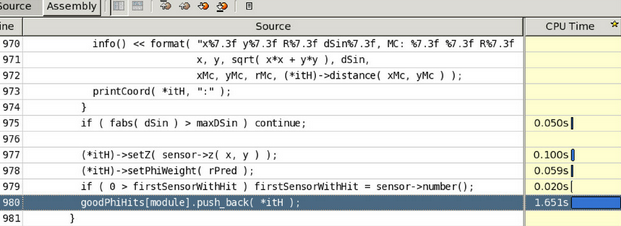
\includegraphics[width=.7\textwidth]{images/cpu03.png}
% \end{frame}

% \begin{frame}
% \frametitle{Event selection criteria}
% \begin{center}
% \begin{tabular}{|l|c|}\hline
% $p_{T}(\Upsilon) > 14$ GeV & todo \\
% $dm \Upsilon(1S) \leq 0.2 GeV$  & todo   \\
% $p_{T}(\gamma) > 0.6 GeV$  &  todo  \\
% $ 0 \leq \chi^{2}_{dtf} \leq 4$  &  todo  \\
% $ lv01 > 0$  &  todo\\ \hline
% \end{tabular}
% \end{center}
% \end{frame}

% \begin{frame}
% \frametitle{Cross sections}
% \begin{enumerate}
%   \item $\Upsilon(1S)$
%     \begin{enumerate}
%       \item $\frac{\sigma(\chi_b(1P) \rightarrow \Upsilon(1S))}{\sigma(\Upsilon(1S))}[p_T(\Upsilon(1S))]$ \textcolor{blue}{IN PROGRESS}
%       \item $\frac{\sigma(\chi_b(2P) \rightarrow \Upsilon(1S))}{\sigma(\Upsilon(1S))}[p_T(\Upsilon(1S))]$
%       \item $\frac{\sigma(\chi_b(3P) \rightarrow \Upsilon(1S))}{\sigma(\Upsilon(1S))}[p_T(\Upsilon(1S))]$
%     \end{enumerate}
%   \item $\Upsilon(2S)$
%     \begin{enumerate}
%       \item $\frac{\sigma(\chi_b(2P) \rightarrow \Upsilon(1S))}{\sigma(\Upsilon(1S))}[p_T(\Upsilon(2S))]$
%       \item $\frac{\sigma(\chi_b(3P) \rightarrow \Upsilon(1S))}{\sigma(\Upsilon(1S))}[p_T(\Upsilon(2S))]$
%     \end{enumerate}
% \item $\Upsilon(3S)$
%     \begin{enumerate}
%       \item $\frac{\sigma(\chi_b(3P) \rightarrow \Upsilon(3S))}{\sigma(\Upsilon(3S))}[Constant]$
%     \end{enumerate}
% \end{enumerate}
% \end{frame}
\end{document}